\section{Laboratory Lecture 6: Safecode}

The aim of this laboratory lecture is to build a system which stores a 4 digit code, which will be entered by the user using a keupad, as we saw in Practice 5 (\textbf{See Section \ref{sec:KEYPAD_GENERAL} for more on this topic}).\medskip

To achieve this, we will use a reprogrammable temporary storage device, i.e. a RAM, which stands for Random Access Memory. Before diving into the laboratory lecture, we will briefly go over the basics of these type of storage devices.


\subsection{Introduction: Random Access Memory}

The auxiliary memory of a system has the duty of keeping essential information that the Central Processing Unit (CPU), in our case a GAL, needs in order to operate correctly.\medskip

This information is usually kept in words of two bytes (16 bits in total), treated as individual entities or memory locations.\medskip

In order to increment the amount of data that can be stored, memory devices usually combine multiple memory locations into two dimensional arrays (i.e. 8x8 array), or even three dimensional arrays (i.e. 8x8x8 array). We can see this here:\medskip

\begin{figure}[H]
    \centering
    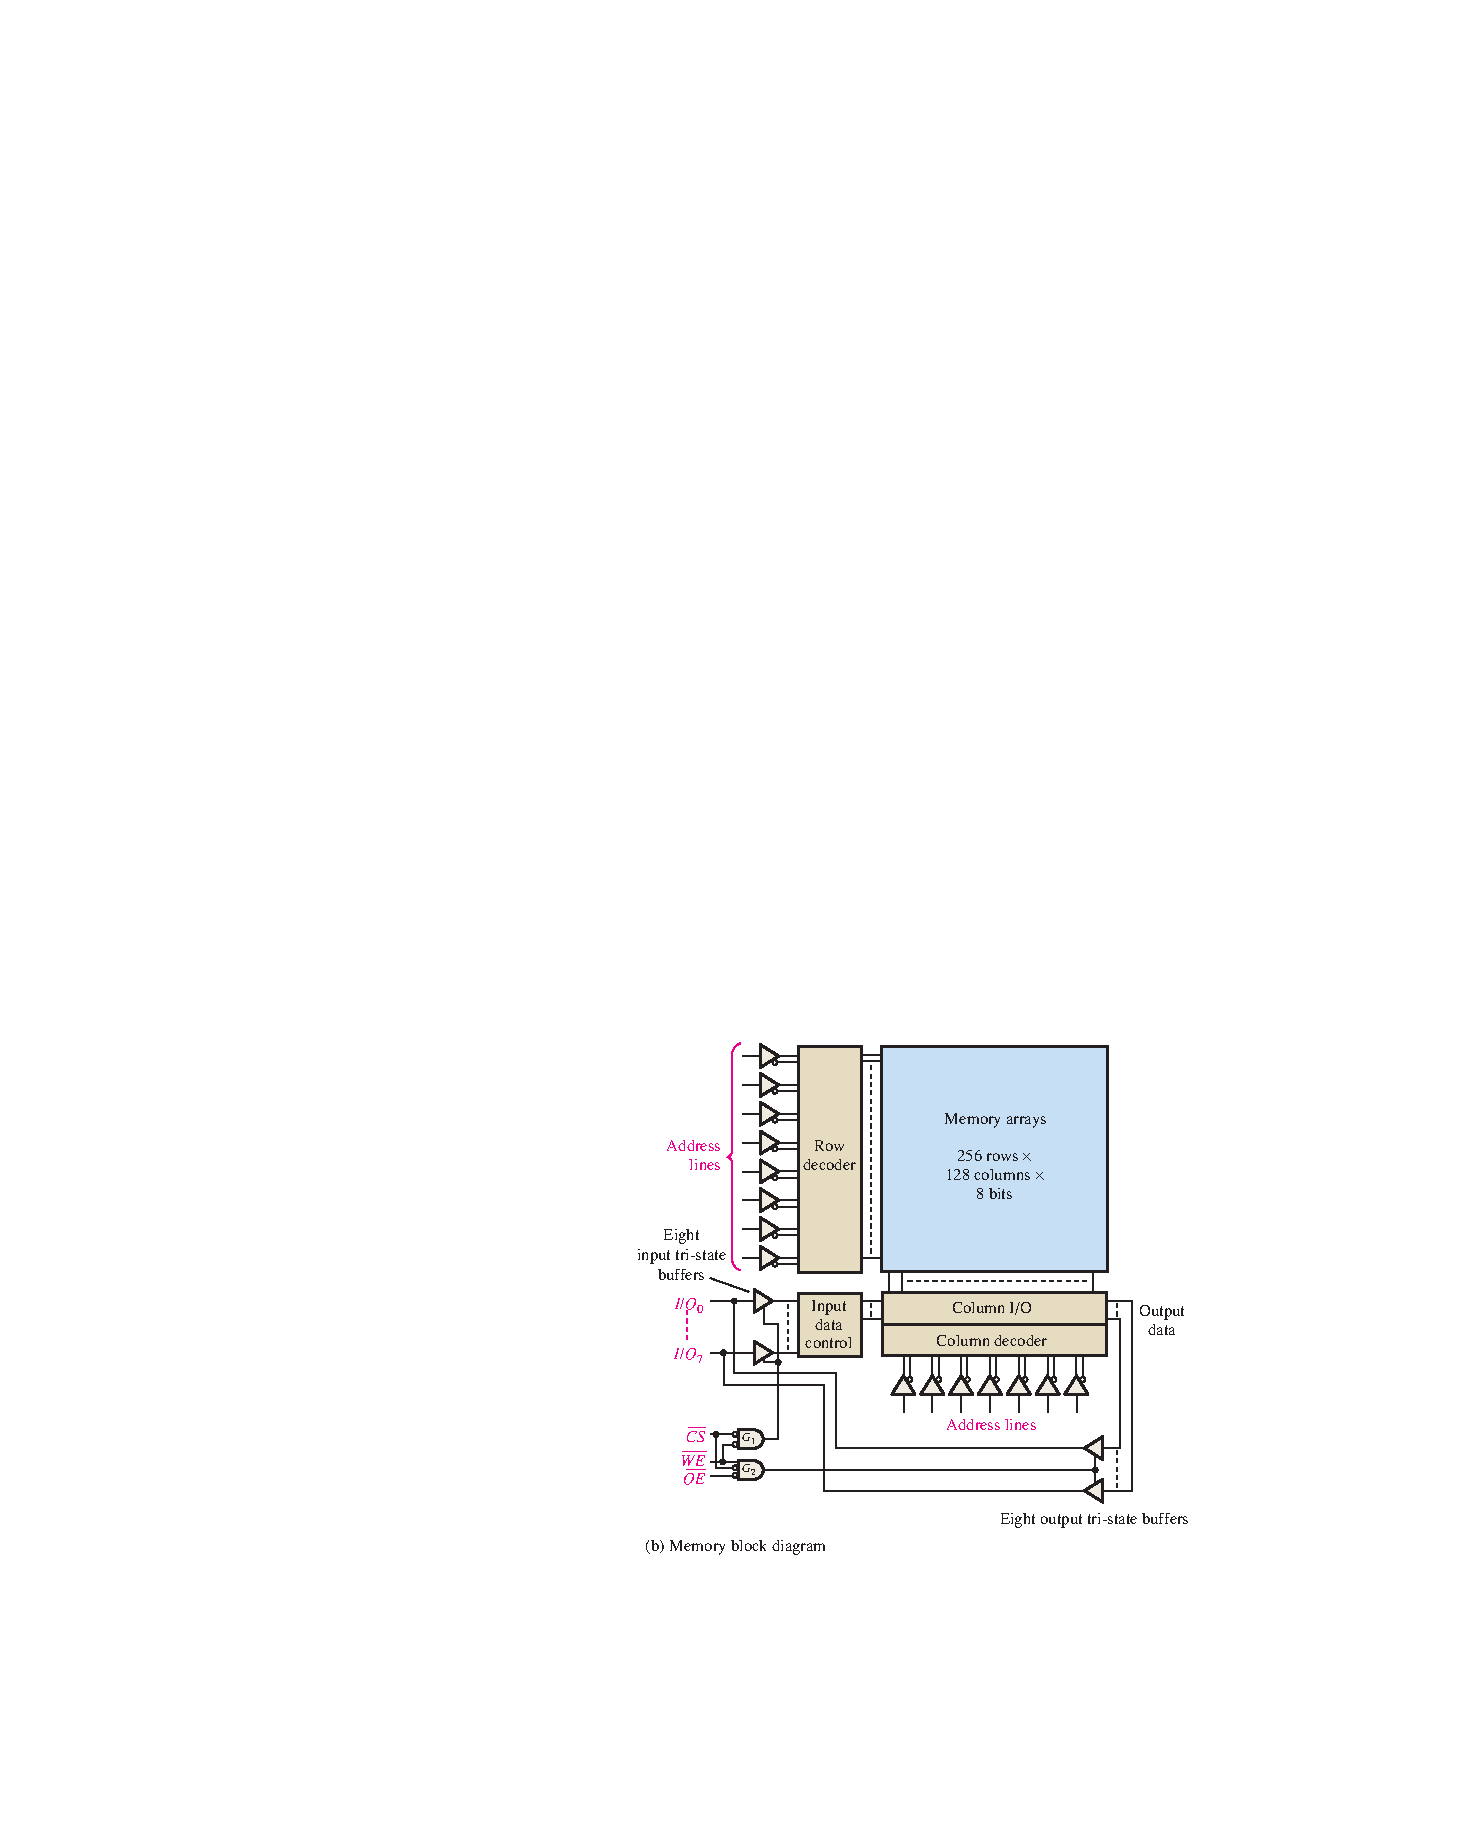
\includegraphics[scale = 0.85]{Graphics/VHDL/Practice 6/RAM/RAM_BLOCK_DIAG.pdf}
    \caption{RAM block diagram ~\autocite{FLOYD}}
    \label{fig:RAM_BLOCK_DIAG}
\end{figure}


\begin{figure}[H]
    \centering
    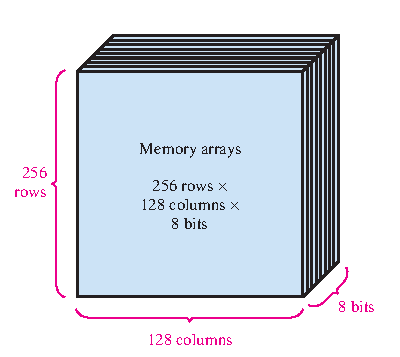
\includegraphics[scale = 0.85]{Graphics/VHDL/Practice 6/RAM/RAM_BLOCK_CONFIG.pdf}
    \caption{RAM array configuration ~\autocite{FLOYD}}
    \label{fig:RAM_BLOCK_CONFIG}
\end{figure}


\subsubsection{Chip description}

Due to its internal structure, most readily available RAMs use the same pinout. In this practice in particular, we have used a 6116, a 16K (2K x 8-bit) Random Access Memory.\medskip

One example of said pinout can be seen below:

\begin{figure}[H]
    \centering
    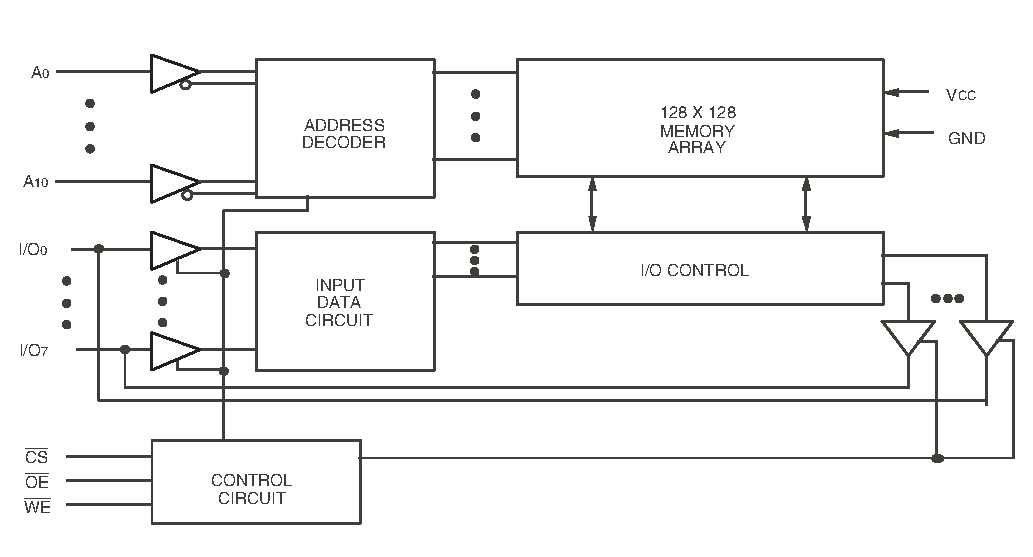
\includegraphics[scale = 0.8]{Graphics/VHDL/Practice 6/RAM/RAM_IO.pdf}
    \caption{6116 RAM Pinout ~\autocite{6116}}
    \label{fig:<label>}
\end{figure}

\clearpage

In the graph, we can clearly distinguish 3 main blocks apart from the storage ones, namely the Address bus, the I/O bus and the Control circuitry.\medskip

The different functions of these blocks are described below:

\paragraph{Control circuitry}

The control of most RAMs is performed by changing the state of 3 pins, namely $\overline{CE}$, $\overline{OE}$, and $\overline{WE}$.\medskip

We will now see what the function of these pins is:\medskip


\textbf{Chip Enable} \medskip

To operate the memory first we have to activate the Chip Enable $\overline{CE}$ terminal (Active Low). \medskip

When a CPU has to handle multiple memory chips, in order to read or write from one of them, the other ones are disabled by sending a HIGH to their respective $\overline{CE}$ terminals. \medskip

\textbf{Write Enable} \medskip

With this terminal the CPU specifies if the operation it wants to execute is to write into the memory (LOW at $\overline{WE}$) or to read from it (HIGH at $\overline{WE}$).\medskip


\textbf{Output enable} \medskip

The $\overline{OE}$ connects the output of the memory to the data bus. If it is in LOW, data can be sent from the memory. Otherwise, a HIGH level will create a High-Z output at the Data Bus.  We usually keep it in a constant LOW in order to simplify the system.\medskip

We can see all of the possible operation modes in the table attached below: 

\begin{table}[H]
    \centering
        \begin{tabular}[t]{lccccc}
            \toprule
            & \textbf{Mode} & $\mathbf{\overline{CS}}$ & $\mathbf{\overline{OE}}$ & $\mathbf{\overline{WE}}$ & \textbf{I/O}\\
            \midrule
                &    Standby   &    H   &   X   &   X   &   High-Z        \\
                &    Read      &    L   &   L   &   H   &   $\text{DATA}_{OUT}$    \\
                &    Read      &    L   &   H   &   H   &   High-Z        \\
                &    Write     &    L   &   X   &   L   &   $\text{DATA}_{IN}$     \\
            \bottomrule
        \end{tabular}
        \caption{Operation Modes Truth Table ~\autocite{6116}}
        \label{table: RAM_MODES}
\end{table}

\clearpage

\paragraph{Address bus}

The Address decoder bus reads the address that the user provides, by pulling the different address pins $\mathbf{\left[ A_0...A_{10} \right]}$ either HIGH or LOW, and it points the memory to that it. In essence, when the user selects an address, depending on the configuration of the control pins, the RAM will either write information to that specific address or read it from it. 


\paragraph{I/O bus}

The I/O bus, as the name suggest is an array of pins that are used to both write information to the RAM or to read from it, depending, again, on the configuration of the Control circuitry. When the RAM is in program mode, i.e. writing mode, the state of these pins will be saved into the address specified by the user. On the other hand, when the RAM is in read mode, the contents of the selected address will appear on this bus.\medskip


In order to simplify the operation, as only 4 digits will be stored, we will only use the $A_0$ and $A_1$ Address terminals. Besides, as we only need to store digits from 0 to 9, only the first 4 bits of the I/O Bus will be used.\medskip

We can see the different pins that we have just discussed in the following image:\medskip

\begin{figure}[H]
    \centering
    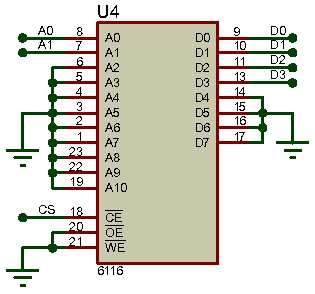
\includegraphics[scale = 1.2]{Graphics/VHDL/Practice 6/RAM/RAM_PROTEUS.PDF}
    \caption{Proteus Subassembly of RAM}
    \label{fig:RAM_PROTEUS_Subassembly}
\end{figure}

\clearpage

\subsection{Exercise 1: Safecode}

Now that we have seen how RAM ICs work, we will move on to the practice itself. As we said before, the aim of this practice is to design and build a system that takes a number, entered by the user using a keypad, and stores it into the RAM for later use. 

\subsubsection{Writing Operation}
\label{sec:WRITING_OPERATION}

In order to be able to both read and store the number, we will use two GALs. One of them will be the one described in the last laboratory lecture (\textbf{See Section \ref{sec:KEYPAD_GENERAL} for more on this topic}) and the other corresponds to the one desgined in this lecture. 

The inputs of this GAL will be:

\begin{itemize}
    \item \textbf{CLK:} Clock input.
    \item \textbf{SIG:} The BCD code coming from the first GAL.
\end{itemize}

On the other hand, the outputs will be:

\begin{itemize}
    \item \textbf{D:} Password output (To program the RAM).
    \item \textbf{CS:} Chip select (To select between Write and Standby Mode)
    \item \textbf{A:} Address (As INOUT) to select the address to which the GAL must write.
\end{itemize}

We can see this in the following image:

\begin{figure}[H]
    \centering
    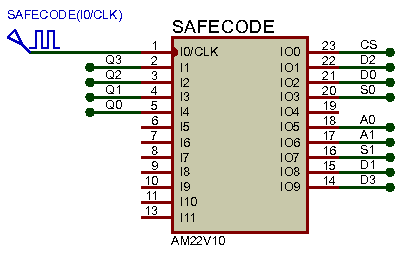
\includegraphics[scale = 1.15]{Graphics/VHDL/Practice 6/SAFECODE/SAFECODE_PROTEUS_GAL.PDF}
    \caption{Proteus Subassembly of Safecode}
    \label{fig:SAFECODE_PROTEUS}
\end{figure}

\clearpage

The memory device will start storing data when the Write Enable ($\overline{WE}$) signal and the Chip Select ($\overline{CS}$) are pulled LOW by the GAL. A timing diagram is attached:\medskip


\begin{figure}[H]
    \centering
    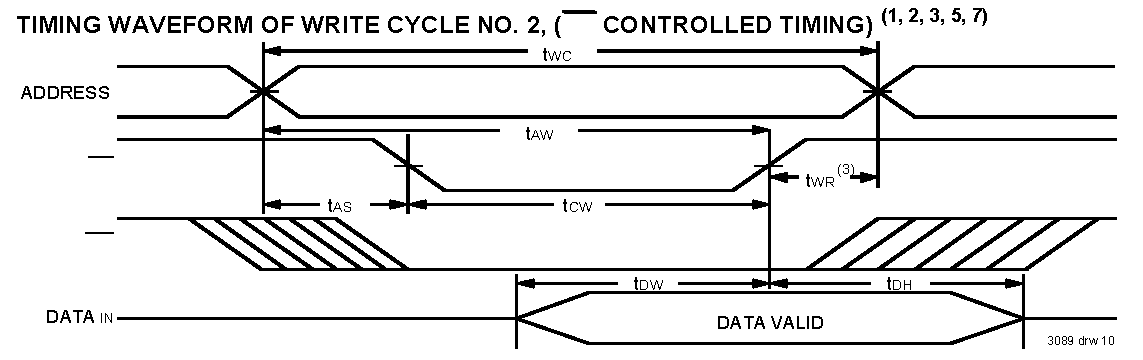
\includegraphics[scale = 0.60]{Graphics/VHDL/Practice 6/RAM/6116.pdf}
    \caption{6116 RAM Write Cycle ~\autocite{6116}}
    \label{fig:6116}
\end{figure}


The general truth table of this specific RAM, though it is mostly the same for most RAM chips, can be found in \textbf{Table} \textbf{\ref{table: RAM_MODES}} \medskip

Now we will discuss the different states that we have defined in our FSM. As per before, the full code will be attached as well.

\subsubsection{FSM States Overview}

\hspace{0.4cm}
    \bm{$Q_0$}
\medskip

At rest, the system must start at Address "00", and the $\overline{CS}$ signal must be pulled HIGH do to it being active LOW. Once the $*$ button is pressed, system transitions to $Q_1$ state.

\medskip
    \bm{$Q_1$}
\medskip

The $\overline{CS}$ signal is pulled LOW level, and the RAM device is in the “ready to write” state $Q_1$. This means that from now on, Address number $00$ is ready to be overwritten by the character we introduce with the keypad. \medskip

When introducing a new character with the keypad, pressing $*$ repeatedly will make the system stay in $Q_1$, pressing the \textit{\#} character will make the system return to $Q_0$, and pressing any other character will make the system change to State $Q_2$. \medskip

\bm{$Q_2$} \textbf{\&} \bm{$Q_3 \textit{\textbf{ and return to }} Q_0$}\medskip

In state $Q_2$, the character previously introduced is written on the address $00$.\medskip

\clearpage

Now, there are two options, either to keep writing to the memory, or to stop writing:

\begin{itemize}
    \item In order to keep writing, any key pressed but \textit{\#} and the \textbf{same key} \footnote{The password cannot contain consecutive digits due to the memory limitations of the GAL. For instance \textit{1212} would be a valid password, but \textit{1122} would not.}, will transition the system to state $Q_3$, where the system jumps to the next Address (where the next character will be kept), and the writing loop starts again at \textit{$Q_1$}.
    
    \item In order to stop, the  \textit{\#} button is pressed, and the system returns to state \textit{$Q_0$}, meaning that  the Address is reset to $00$, and the writing operation ends.
\end{itemize}


To illustrate the different states and the transitions between them we have included the following diagram:\medskip

\begin{figure}[H]
    \centering
    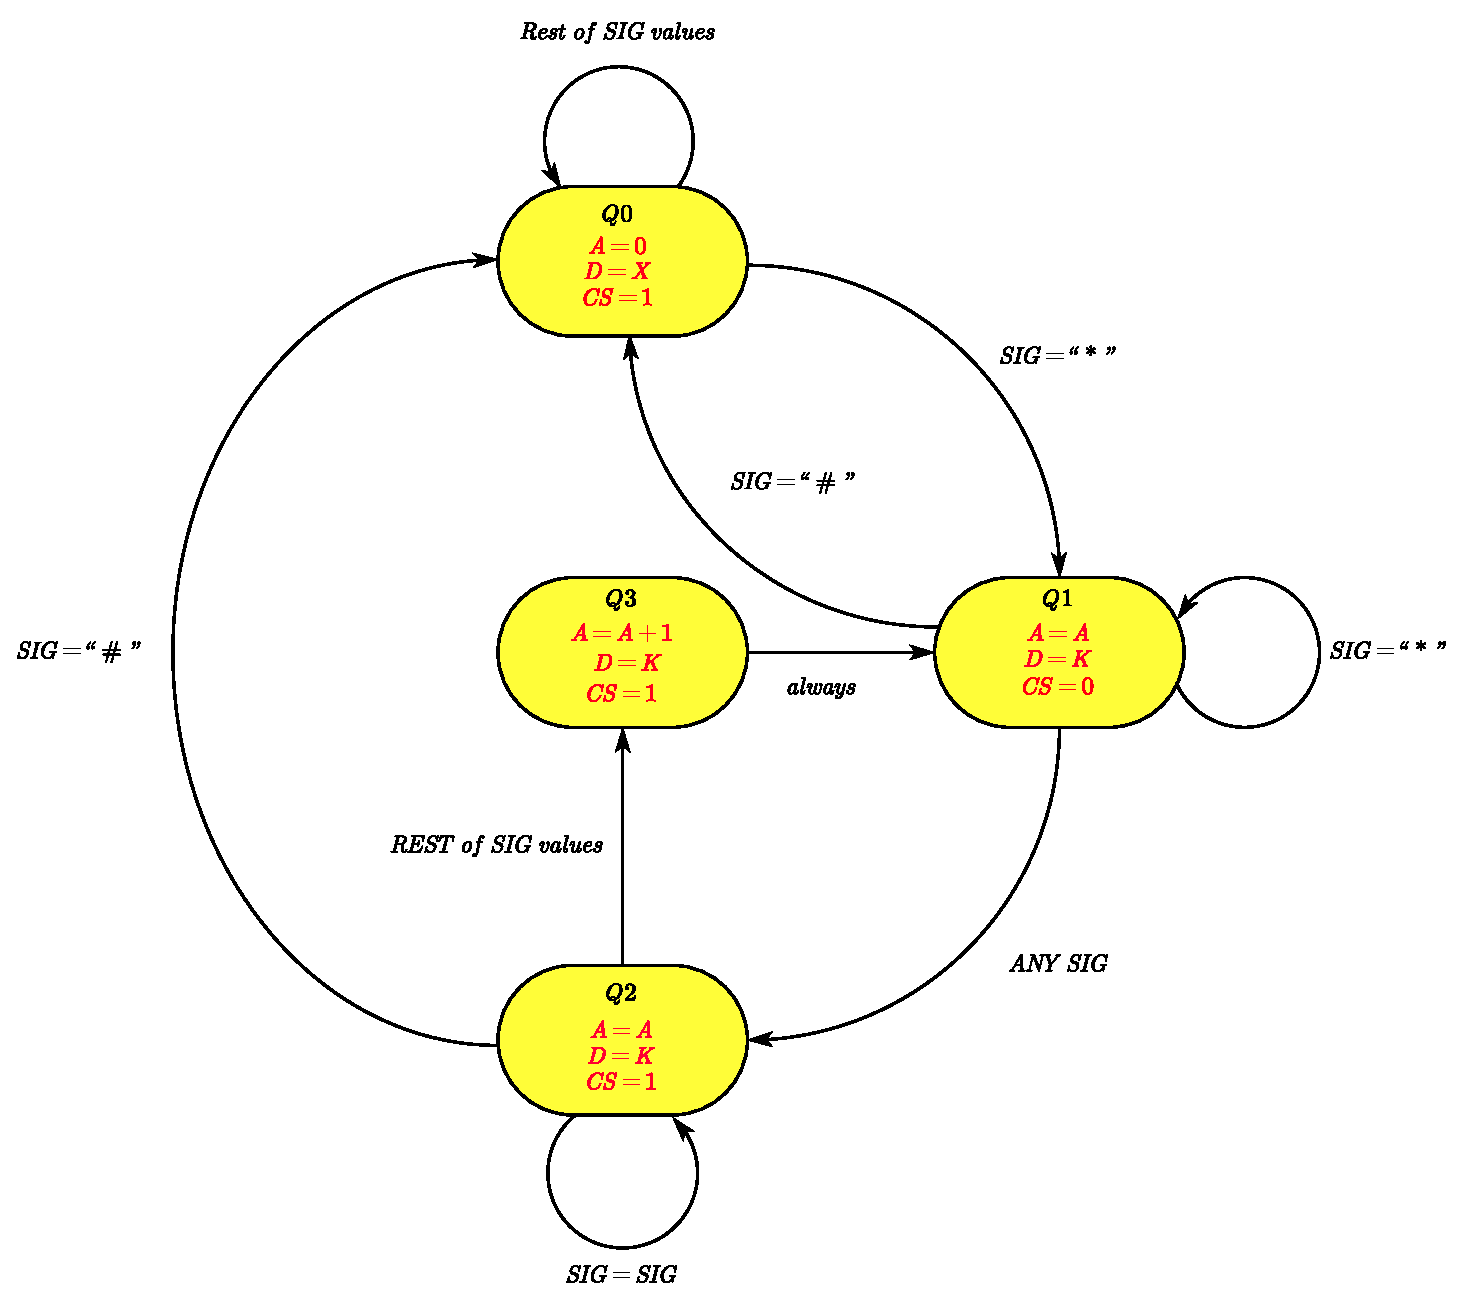
\includegraphics[scale = 0.55]{Graphics/VHDL/Practice 6/SAFECODE/SAFECODE_FSM.pdf}
    \caption{Safecode FSM}
    \label{fig:SAFECODE_FSM}
\end{figure}

\clearpage

The VHDL code for this GAL can be found below:

\inputcode{CODES/VHDL/Practice_6/SAFECODE.vhd}

The final Proteus assembly can be found below:

\begin{figure}[H]
    \centering
 
    \ifnum\value{ANIMATION}=1 {
        \animategraphics[controls,loop,scale=0.78]{1}{Graphics/VHDL/Practice 6/SAFECODE/ANIMATION/F}{0}{5}
    } 
    \else {
        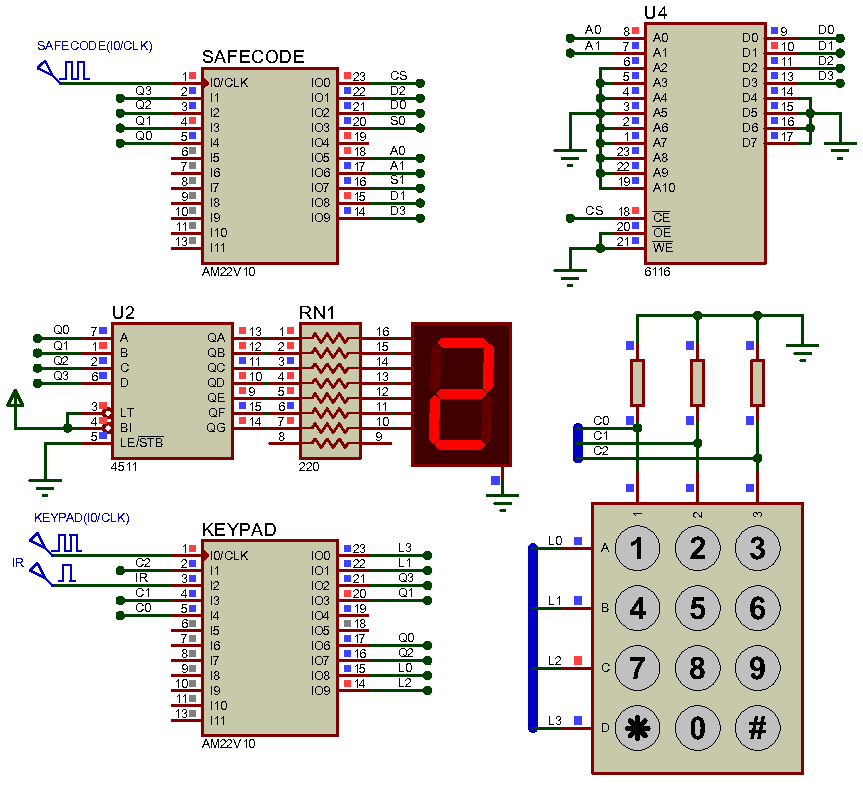
\includegraphics[scale=0.78]{Graphics/VHDL/Practice 6/SAFECODE/ANIMATION/F2.pdf}
    }\fi
    
    \caption{Proteus Assembly of Safecode}
    \label{fig:PROTEUS_SAFECODE_ASSEMBLY_FINAL}
\end{figure}
            
After introducing the code, we can pause the simulation and check that indeed, the "Memory Contents" pop-up window displays the entered data.\medskip

\begin{table}[H]
    \centering
        \begin{tabular}[t]{lccccc}
            \toprule
                &\multicolumn{5}{c}{\textbf{Memory Contents}}\\
                & 0000 & 01 & 02 & 03 & 04 \\
            \bottomrule
        \end{tabular}
        \caption{RAM Contents}
        \label{table:RAM_CONTENTS}
\end{table}

\clearpage
















